%-----------------------------------------------------------------------------------------------------------------------------------------------%
%	The MIT License (MIT)
%
%	Copyright (c) 2015 Jan Küster
%
%	Permission is hereby granted, free of charge, to any person obtaining a copy
%	of this software and associated documentation files (the "Software"), to deal
%	in the Software without restriction, including without limitation the rights
%	to use, copy, modify, merge, publish, distribute, sublicense, and/or sell
%	copies of the Software, and to permit persons to whom the Software is
%	furnished to do so, subject to the following conditions:
%	
%	THE SOFTWARE IS PROVIDED "AS IS", WITHOUT WARRANTY OF ANY KIND, EXPRESS OR
%	IMPLIED, INCLUDING BUT NOT LIMITED TO THE WARRANTIES OF MERCHANTABILITY,
%	FITNESS FOR A PARTICULAR PURPOSE AND NONINFRINGEMENT. IN NO EVENT SHALL THE
%	AUTHORS OR COPYRIGHT HOLDERS BE LIABLE FOR ANY CLAIM, DAMAGES OR OTHER
%	LIABILITY, WHETHER IN AN ACTION OF CONTRACT, TORT OR OTHERWISE, ARISING FROM,
%	OUT OF OR IN CONNECTION WITH THE SOFTWARE OR THE USE OR OTHER DEALINGS IN
%	THE SOFTWARE.
%	
%
%-----------------------------------------------------------------------------------------------------------------------------------------------%

%============================================================================%
%
%	DOCUMENT DEFINITION
%
%============================================================================%

%we use article class because we want to fully customize the page and dont use a cv template
\documentclass[11pt,A4]{article}	

%----------------------------------------------------------------------------------------
%	ENCODING
%----------------------------------------------------------------------------------------

%we use utf8 since we want to build from any machine
\usepackage[utf8]{inputenc}
\usepackage[vietnamese]{babel}

%----------------------------------------------------------------------------------------
%	LOGIC
%----------------------------------------------------------------------------------------

% provides \isempty test
\usepackage{xifthen}

%----------------------------------------------------------------------------------------
%	FONT
%----------------------------------------------------------------------------------------

% some tex-live fonts - choose your own

\usepackage[defaultsans]{droidsans}
%\usepackage[default]{comfortaa}
%\usepackage{cmbright}
%\usepackage[default]{raleway}
%\usepackage{fetamont}
%\usepackage[default]{gillius}
%\usepackage[light,math]{iwona}
%\usepackage[thin]{roboto} 

% set font default
\renewcommand*\familydefault{\rmdefault} 	
\usepackage[T1]{fontenc}

% more font size definitions
\usepackage{moresize}		

%\usepackage[fixed]{fontawesome5}
\usepackage{fontawesome5}

\usepackage{hyperref}

%----------------------------------------------------------------------------------------
%	PAGE LAYOUT  DEFINITIONS
%----------------------------------------------------------------------------------------

%debug page outer frames
%\usepackage{showframe}			

%define page styles using geometry
\usepackage[a4paper]{geometry}		

% for example, change the margins to 2 inches all round
%\geometry{top=1cm, bottom=-.6cm, left=0.4cm, right=1cm}
\geometry{top=0.7cm, bottom=-1.8cm, left=0cm, right=0.55cm}

%less space between header and content
\setlength{\headheight}{-5pt}		

%customize entries left, center and right
%\lhead{}
%\chead{ \small{Jan Küster  $\cdot$ Consultant and Software Engineer $\cdot$  Bremen, Germany  $\cdot$  \textcolor{sectcol}{\textbf{info@jankuester.com}}  $\cdot$ +49 176 313 *** **}}
%\rhead{}

%indentation is zero
\setlength{\parindent}{0mm}

%----------------------------------------------------------------------------------------
%	TABLE /ARRAY DEFINITIONS
%---------------------------------------------------------------------------------------- 

%for layouting tables
\usepackage{multicol}			
\usepackage{multirow}

%extended aligning of tabular cells
\usepackage{array}

\newcolumntype{x}[1]{%
>{\raggedleft\hspace{0pt}}p{#1}}%

%----------------------------------------------------------------------------------------
%	GRAPHICS DEFINITIONS
%---------------------------------------------------------------------------------------- 

%for header image
\usepackage{graphicx}

%for floating figures
\usepackage{wrapfig}
\usepackage{float}
%\floatstyle{boxed} 
%\restylefloat{figure}

%for drawing graphics		
\usepackage{tikz}				
\usetikzlibrary{shapes, backgrounds,mindmap, trees}

%----------------------------------------------------------------------------------------
%	Color DEFINITIONS
%---------------------------------------------------------------------------------------- 
\usepackage{transparent}
\usepackage{color}

%accent color
\definecolor{complcol}{RGB}{250,150,10}

%dark background color
\definecolor{bgcol}{RGB}{110,110,110}

%light background / accent color
\definecolor{softcol}{RGB}{225,225,225}

\definecolor{sectcol}{RGB}{0,120,150}

%============================================================================%
%
%
%	DEFINITIONS
%
%
%============================================================================%

% returns minipage width minus two times \fboxsep
% to keep padding included in width calculations
\newcommand{\mpwidth}{\linewidth-\fboxsep-\fboxsep}
	
%----------------------------------------------------------------------------------------
% 	ARROW GRAPHICS in Tikz
%----------------------------------------------------------------------------------------

% a six pointed arrow poiting to the left
\newcommand{\tzlarrow}{(0,0) -- (0.2,0) -- (0.3,0.2) -- (0.2,0.4) -- (0,0.4) -- (0.1,0.2) -- cycle;}	

% include the left arrow into a tikz picture
% param1: fill color
%
\newcommand{\larrow}[1]
{\begin{tikzpicture}[scale=0.58]
	 \filldraw[fill=#1!100,draw=#1!100!black]  \tzlarrow
 \end{tikzpicture}
}

% a six pointed arrow poiting to the right
\newcommand{\tzrarrow}{ (0,0.2) -- (0.1,0) -- (0.3,0) -- (0.2,0.2) -- (0.3,0.4) -- (0.1,0.4) -- cycle;}

% include the right arrow into a tikz picture
% param1: fill color
%
\newcommand{\rarrow}
{\begin{tikzpicture}[scale=0.7]
	\filldraw[fill=sectcol!100,draw=sectcol!100!black] \tzrarrow
 \end{tikzpicture}
}

%----------------------------------------------------------------------------------------
%	custom sections
%----------------------------------------------------------------------------------------

% create a coloured box with arrow and title as cv section headline
% param 1: section title
%
\newcommand{\cvsection}[1]
{
\colorbox{sectcol}{\mystrut \makebox[1\mpwidth][l]{
\larrow{bgcol} \hspace{-8pt} \larrow{bgcol} \hspace{-8pt} \larrow{bgcol} \textbf{\textcolor{white}{\uppercase{#1}}}\hspace{4pt}
}}\\
}

% create a coloured arrow with title as cv meta section section
% param 1: meta section title
%
\newenvironment{metasection}[1] {
	%\vspace{2pt}
	\begin{center}
		\textbf{\textcolor{white}{\large{\uppercase{#1}}}}\\[-4pt]
	\normalsize
	\parbox{0.7\mpwidth}{\textcolor{white}	\hrule}\\
}{\end{center}}

%----------------------------------------------------------------------------------------
%	 CV EVENT
%----------------------------------------------------------------------------------------

% creates a stretched box as cv entry headline followed by two paragraphs about 
% the work you did
% param 1:	event time i.e. 2014 or 2011-2014 etc.
% param 2:	event name (what did you do?)
% param 3:	institution (where did you work / study)
% param 4:	what was your position
% param 5:	some words about your contributions
%
\newcommand{\cvevent}[5]
{
\vspace{8pt}
	\begin{tabular*}{1\mpwidth}{p{0.35\mpwidth}  x{0.62\mpwidth}}
	% The sum of the two coefficients above must be 0.97
 	\textcolor{black}{\textbf{#2}} & \textcolor{complcol}{#3} | \textcolor{bgcol}{#1} 

	\end{tabular*}
\vspace{-12pt}
\textcolor{softcol}{\hrule}
\vspace{6pt}
	\begin{tabular*}{0.5\mpwidth}{p{\mpwidth}}
\larrow{softcol}  #4\\[3pt]
\larrow{softcol}  #5\\[6pt]
	\end{tabular*}
}

% creates a stretched box as 
\newcommand{\cveventmeta}[2]
{
	\mbox{\mystrut \hspace{87pt}\textit{#1}}\\
	#2
}

\newcommand{\boldwhite}[1]
{
\textcolor{white}{\textbf{#1}}
}

%----------------------------------------------------------------------------------------
% CUSTOM STRUT FOR EMPTY BOXES
%----------------------------------------- -----------------------------------------------
\newcommand{\mystrut}{\rule[-.3\baselineskip]{0pt}{\baselineskip}}

%----------------------------------------------------------------------------------------
% CUSTOM LOREM IPSUM
%----------------------------------------------------------------------------------------
\newcommand{\lorem}
{Lorem ipsum dolor sit amet, consectetur adipiscing elit. Donec a diam lectus.}

% use to vertically center content
% credits to: http://tex.stackexchange.com/questions/7219/how-to-vertically-center-two-images-next-to-each-other
\newcommand{\vcenteredinclude}[1]{\begingroup
\setbox0=\hbox{\includegraphics{#1}}%
\parbox{\wd0}{\box0}\endgroup}

% use to vertically center content
% credits to: http://tex.stackexchange.com/questions/7219/how-to-vertically-center-two-images-next-to-each-other
\newcommand*{\vcenteredhbox}[1]{\begingroup
\setbox0=\hbox{#1}\parbox{\wd0}{\box0}\endgroup}

%----------------------------------------------------------------------------------------
%	ICON-SET EMBEDDING
%---------------------------------------------------------------------------------------- 

% at this point we simplify our icon-embedding by simply referring to a set of png images.
% if you find a good way of including svg without conflicting with other packages you can
% replace this part
\newcommand{\icon}[3]{\makebox(#2, #2){\vspace*{2pt} \textcolor{#3}{\csname fa#1\endcsname}}}	%icon shortcut
\newcommand{\icontext}[4]{ 						%icon with text shortcut
	\vcenteredhbox{\icon{#1}{#2}{#4}} \vcenteredhbox{ \textcolor{#4}{#3}}
}

%============================================================================%
%
%
%
%	DOCUMENT CONTENT
%
%
%
%============================================================================%

\begin{document}
\fcolorbox{white}{white}{\begin{minipage}[c][0.95\textheight][t]{0.75\linewidth}

%---------------------------------------------------------------------------------------
%	TITLE HEADLINE
%----------------------------------------------------------------------------------------
\vspace{-3pt}
% use this for multiple words like working titles etc.
\colorbox{sectcol}{
    \makebox[\mpwidth-2.55mm][l]{
        \hspace{3pt}\HUGE{\textcolor{white}{\uppercase{Vincent Le Goualher}}}
        \textcolor{white}{\rule[-1mm]{1mm}{0.9cm}}
        \parbox[b]{2cm}{
            \large{ \textcolor{white}{{\textbf{Data}}}}\\
            \large{ \textcolor{white}{{\textbf{Scientist}}}}}
    }
}

% use this for single words, e.g. CV or RESUME etc.
%\colorbox{bgcol}{\makebox[\mpwidth][c]{\HUGE{\textcolor{white}{\uppercase{Vincent Le Goualher}} }  }}

%----------------------------------------------------------------------------------------
%	HEADER IMAGE
%----------------------------------------------------------------------------------------

%\hspace{-1.6cm}
%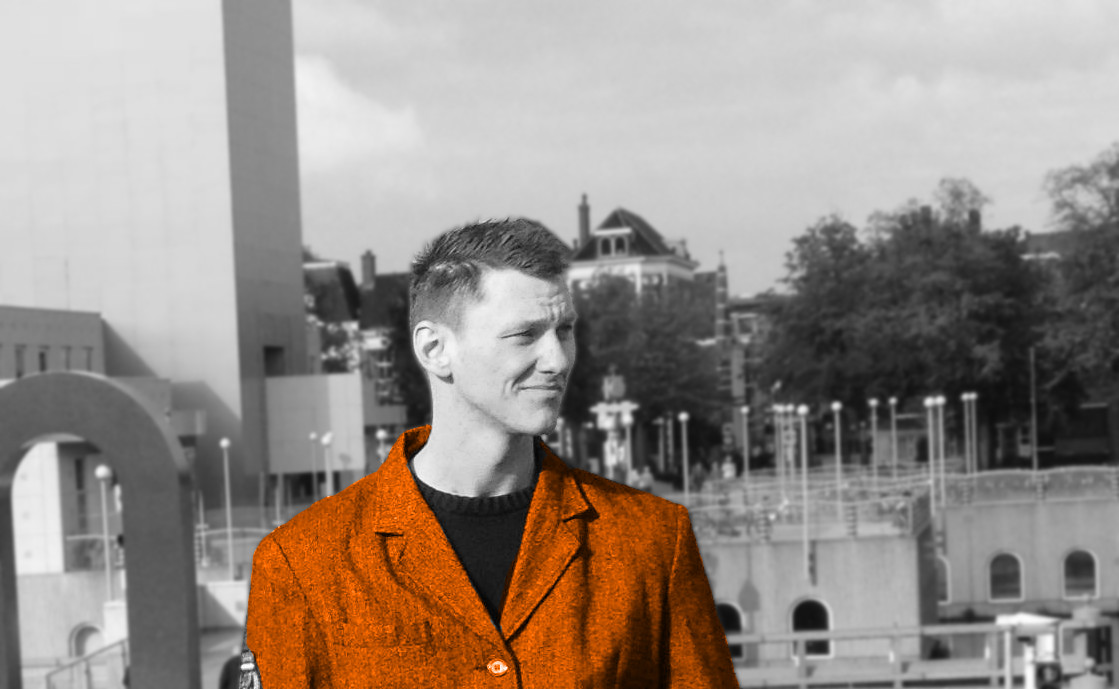
\includegraphics[trim= 0 250 0 270,clip,width=1\linewidth+3.1cm]{myfoto.jpg}	%trimming relative to image size!
\includegraphics[trim= 300 1300 0 650, clip ,width=\linewidth]{cv_gentil_1_face.jpeg}	%trimming relative to image size
%\includegraphics[trim= 30 130 0 40, clip ,width=\linewidth]{cool_1.jpeg}

%---------------------------------------------------------------------------------------
%	SUMMARY
%----------------------------------------------------------------------------------------
\transparent{0.80}%
\vspace{-112pt}
\hspace{0.32\linewidth}
\colorbox{bgcol}{
	\parbox{0.58\linewidth}{
		\transparent{1}%
		\begin{center}
		\larrow{sectcol}\larrow{sectcol}\textcolor{white}{Passionate about statistics and machine learning, I have been analysing data and developing models for two years in order to solve problems in various industries.}
		\end{center}
	}
}
\vspace{32.5pt}

\transparent{0.90}%

%============================================================================%
%
%	CV SECTIONS AND EVENTS (MAIN CONTENT)
%
%============================================================================%

%---------------------------------------------------------------------------------------
%	STATUS
%----------------------------------------------------------------------------------------
%\cvsection{Status}

%JavaScript fullstack engineer, M.Sc. Digital Media, focuses on education and healthcare

%\vspace{12pt}

%---------------------------------------------------------------------------------------
%	EXPERIENCE
%----------------------------------------------------------------------------------------

\cvsection{Experience}

%CCLS
\vspace{6pt}
    \begin{tabular*}{1\mpwidth}{p{0.35\mpwidth}  x{0.62\mpwidth}}
    \textcolor{black}{\textbf{Data Scientist}} & \textcolor{complcol}{\href{https://www.creditmutuel-leasing.eu/en/index.html}{\underline{CM-CIC Leasing Solutions}}, Paris} | \textcolor{bgcol}{06/2019 - ../....}

    \end{tabular*}
\vspace{-12pt}
\textcolor{softcol}{\hrule}
\vspace{6pt}
    \begin{tabular*}{0.5\mpwidth}{p{\mpwidth}}
\larrow{softcol}  Worked on residual value forecasting in order to better contract pricing\\[3pt]
\larrow{softcol}  Built a classifier to list business introducers. Improved usability of previous model and\\
\hspace{0.33cm} increased accuracy by 15 \% using random forest algorithm\\[3pt]
\larrow{softcol}  Estimated the cost of material failures with survival analysis for recurrent events\\[3pt]
\larrow{softcol}  Developed an anomaly detection module for the compliance department using \href{https://en.wikipedia.org/wiki/Local_outlier_factor}{\underline{LOF}},\\
\hspace{0.33cm} which led to partially automate the process of identifying irregularities\\[6pt]
    \end{tabular*}

% Grandmont
\vspace{6pt}
    \begin{tabular*}{1\mpwidth}{p{0.25\mpwidth}  x{0.72\mpwidth}}
    \textcolor{black}{\textbf{Math Teacher}} & \textcolor{complcol}{Secondary school Grandmont, Tours (FR)} | \textcolor{bgcol}{09/2017 - 03/2019}

    \end{tabular*}
\vspace{-12pt}
\textcolor{softcol}{\hrule}
\vspace{6pt}

% PT
\vspace{6pt}
    \begin{tabular*}{1\mpwidth}{p{0.40\mpwidth}  x{0.57\mpwidth}}
    \textcolor{black}{\textbf{Math/English Teacher}} & \textcolor{complcol}{Phan Thiết, Việt Nam} | \textcolor{bgcol}{Q1/2014 - 08/2016}

    \end{tabular*}
\vspace{-12pt}
\textcolor{softcol}{\hrule}
\vspace{6pt}

% Hardis
\vspace{6pt}
    \begin{tabular*}{1\mpwidth}{p{0.35\mpwidth}  x{0.62\mpwidth}}
    \textcolor{black}{\textbf{Software Developer Intern}} & \textcolor{complcol}{\href{https://www.hardis-group.com/}{\underline{Hardis}}, Nantes (FR)} | \textcolor{bgcol}{02/2013 - 08/2013}

    \end{tabular*}
\vspace{-12pt}
\textcolor{softcol}{\hrule}
\vspace{6pt}
    \begin{tabular*}{0.5\mpwidth}{p{\mpwidth}}
\larrow{softcol}  Developed the Android blood sugar tracker app \textsuperscript{\textcopyright}\href{https://www.hardis-group.com/en/news/mobidiab-free-mobile-app-monitoring-diabetes}{\underline{MobiDiab}}\\[3pt]
\larrow{softcol}  Oversaw the project from start to finish : design/specification/implementation/testing\\[6pt]
    \end{tabular*}
    
\vspace{6pt}

%---------------------------------------------------------------------------------------
%	EDUCATION SECTION
%--------------------------------------------------------------------------------------

\cvsection{Education}

% ISUP
\vspace{6pt}
    \begin{tabular*}{1\mpwidth}{p{0.35\mpwidth}  x{0.62\mpwidth}}
    \textcolor{black}{\href{https://sites.google.com/view/isup-isds/accueil?authuser=0}{\underline{\textbf{M. Sc. in Statistics \& Data Science}}}} & \textcolor{complcol}{\href{http://isup.sorbonne-universite.fr/fr/index.html}{\underline{ISUP}}, Paris} | \textcolor{bgcol}{2019 - 2020}

    \end{tabular*}
\vspace{-12pt}
\textcolor{softcol}{\hrule}
\vspace{6pt}
    \begin{tabular*}{0.5\mpwidth}{p{\mpwidth}}
\larrow{softcol}  Theory : deep learning, machine learning, time series, survival analysis, advanced stats\\[3pt]
\larrow{softcol}  Practice : projects available in this \href{https://github.com/datatrigger/school_projects}{\underline{repository}}\\[6pt]
    \end{tabular*}

% CAPES
\vspace{6pt}
    \begin{tabular*}{1\mpwidth}{p{0.40\mpwidth}  x{0.57\mpwidth}}
    \href{https://en.wikipedia.org/wiki/Certificate_of_aptitude_for_secondary_school_teachers_(France)}{\textcolor{black}{\textbf{\underline{Math Education Certification}}}} & \textcolor{complcol}{Tours (FR)} | \textcolor{bgcol}{2017}

    \end{tabular*}
\vspace{-12pt}
\textcolor{softcol}{\hrule}
\vspace{6pt}
    \begin{tabular*}{0.5\mpwidth}{p{\mpwidth}}
\larrow{softcol}  Integration, probability theory, algebra, differential calculus, complex analysis\\[6pt]
    \end{tabular*}

% IMT
\vspace{6pt}
    \begin{tabular*}{1\mpwidth}{p{0.35\mpwidth}  x{0.62\mpwidth}}
    \textcolor{black}{\href{https://www.imt-atlantique.fr/en/study/engineering}{\underline{\textbf{M. Sc. in Engineering}}}} & \textcolor{complcol}{\href{https://www.imt-atlantique.fr/en}{\underline{IMT Atlantique}} (ex-EMN), Nantes (FR)} | \textcolor{bgcol}{2010 - 2013}

    \end{tabular*}
\vspace{-12pt}
\textcolor{softcol}{\hrule}
\vspace{6pt}
    \begin{tabular*}{0.5\mpwidth}{p{\mpwidth}}
\larrow{softcol}  Computer science : Java/C++/SQL/Bash, software architecture, agile development\\[3pt]
\larrow{softcol}  Emphasis on project management and teamwork | 3-month internship in Vietnam\\[6pt]
    \end{tabular*}

% Bachelor
\vspace{6pt}
    \begin{tabular*}{1\mpwidth}{p{0.40\mpwidth}  x{0.57\mpwidth}}
    \href{https://en.wikipedia.org/wiki/Classe_pr\%C3\%A9paratoire_aux_grandes_\%C3\%A9coles\#Scientific_CPGE}{\textcolor{black}{\textbf{\underline{Bachelor of Mathematics}}}} & \textcolor{complcol}{Rennes (FR)} | \textcolor{bgcol}{2008 - 2010}

    \end{tabular*}
\vspace{-12pt}
\textcolor{softcol}{\hrule}
\vspace{6pt}

\vspace{6pt}

%---------------------------------------------------------------------------------------
%	HOBBY SECTION
%--------------------------------------------------------------------------------------

\cvsection{Volunteer work}
    \begin{tabular*}{0.5\mpwidth}{p{\mpwidth}}
\vspace{1pt}
\larrow{softcol} \href{https://github.com/apaad}{\underline{Statistician}} for the French Society of Professional Home Birth Care (\href{https://www.apaad.fr/}{\underline{\textit{APAAD}}})\\[6pt]
%\larrow{softcol} GNU/Linux, German, drums and of course, heavy metal \hspace{-2pt} \icon{Heart}{4}{black}
	\end{tabular*}
	
\vspace{8pt}

%---------------------------------------------------------------------------------------
%	REFERENCE SECTION
%--------------------------------------------------------------------------------------

\cvsection{References \& Diplomas}

%\vspace{-6pt} \ \\
%Mes \textbf{références} et copies de \textbf{diplômes} sont disponibles sur demande.

\begin{tabular*}{0.5\mpwidth}{p{\mpwidth}}
\larrow{softcol} \href{https://www.linkedin.com/in/paul-coudret-885922119/}{\underline{Paul Coudret}}, current manager at \href{https://www.creditmutuel-leasing.eu/en/index.html}{\underline{CM-CIC Leasing Solutions}}\\[6pt]
\larrow{softcol} \href{http://www.floriane-stauffer-sage-femme.com/}{\underline{Floriane Stauffer-Obrecht}}, president of the above-mentioned society (\href{https://www.apaad.fr/}{\underline{\textit{APAAD}}})\\[6pt]
\larrow{softcol} \href{https://www.lpsm.paris/pageperso/broniatowski/}{\underline{Michel Broniatowski}}, chairman of the Department of Statistics \& Data Science (\href{http://isup.sorbonne-universite.fr/fr/index.html}{\underline{ISUP}})\\[6pt]
\larrow{softcol} Copies of my diplomas are available in this \href{https://github.com/datatrigger/diplomas_certificates}{\underline{repository}}
\end{tabular*}

\end{minipage}}
\hspace{-0.2cm}
\fcolorbox{white}{sectcol}{\begin{minipage}[c][0.95\textheight][t]{0.25\linewidth}

%----------------------------------------------------------------------------------------
%	META SECTION
%----------------------------------------------------------------------------------------

\vspace{14pt}

% CONTACT
\begin{metasection}{Contact}%\\[6pt]

	    \icontext{MapMarker}{12}{Paris, France}{white}\\[6pt]
	    %\icontext{AddressCard}{12}{French citizenship}{white}\\[6pt]
	    \icontext{Passport}{12}{French citizenship}{white}\\[6pt]
	    \icontext{Envelope}{12}{\href{mailto:contact@datatrigger.org}{\underline{contact@datatrigger.org}}}{white}\\[6pt]
	    \icontext{MousePointer}{12}{\href{https://www.datatrigger.org}{\underline{www.datatrigger.org}}}{white}\\[6pt]
	    \icontext{Github}{12}{\href{https://github.com/datatrigger}{\underline{github.com/datatrigger}}}{white}\\[6pt]
	    \icontext{Linkedin}{12}{\href{https://www.linkedin.com/in/datatrigger/}{\underline{\small{linkedin.com/in/datatrigger}}}}{white}

\end{metasection}

\vspace{-6pt}

% SKILLS
\begin{metasection}{Skills}
    \vspace{-12pt}
    \begin{flushleft}
        \icontext{CaretRight}{12}{Machine Learning}{white}\\[6pt]
        \icontext{CaretRight}{12}{Deep Learning}{white}\\[6pt]
        \icontext{CaretRight}{12}{Computer Vision}{white}\\[6pt]
        \icontext{CaretRight}{12}{Distributed Computing}{white}\\[6pt]
        \icontext{CaretRight}{12}{Data Visualization}{white}\\[6pt]
        %\icontext{CaretRight}{12}{Clustering}{white}\\[6pt]
        \icontext{CaretRight}{12}{Model Explainability}{white}\\[6pt]
        \icontext{CaretRight}{12}{Reliability}{white}\\[6pt]
        \icontext{CaretRight}{12}{Desc. \& Inf. Statistics}{white}\\[6pt]
        
        % \icontext{CaretRight}{12}{Feature Selection /}{white}\\
        % \textcolor{white}{\hspace{0.4cm} Dimensionality Reduction}\\[6pt]
    \end{flushleft}
\end{metasection}

\vspace{-6pt}

% TOOLS
\begin{metasection}{Tools}
    \icontext{Python}{12}{\textbf{Python}}{white}
    \begin{flushleft}
        \icontext{CaretRight}{12}{Pandas/PySpark}{white}\\[6pt]
        %\icontext{CaretRight}{12}{Plotly/Dash/GraphX}{white}\\[6pt]
        \icontext{CaretRight}{12}{scikit-learn/MLlib}{white}\\[6pt]
        \icontext{CaretRight}{12}{PyTorch/fastai}{white}\\[6pt]
        %\icontext{CaretRight}{12}{TensorFlow/Keras}{white}\\[6pt]
        \icontext{CaretRight}{12}{SHAP}{white}\\[6pt]
    \end{flushleft}
    \icontext{RProject}{12}{}{white}
    \begin{flushleft}
        \icontext{CaretRight}{12}{The Tidyverse}{white}\\[6pt]
        \icontext{CaretRight}{12}{ggplot2/Shiny}{white}\\[6pt]
        \icontext{CaretRight}{12}{stats/caret/survival...}{white}\\[6pt]
    \end{flushleft}
    \icontext{Code}{12}{\textbf{Others}}{white}
    \begin{flushleft}
        \hspace{-1pt}\icontext{Database}{12}{SQL}{white}\\[6pt]
        \hspace{-1pt}\icontext{Cloud}{12}{AWS EC2, SageMaker}{white}\\[6pt]
        \hspace{-1pt}\icontext{Code}{12}{Git/Bash}{white}\\[6pt]
        % Icons ideas : Pen / Edit / File
        \hspace{-1pt}\icontext{Pen}{12}{Markdown/\LaTeX}{white}
    \end{flushleft}
\end{metasection}

\vspace{-6pt}

% LANGUAGES
\begin{metasection}{Languages}

\textcolor{white}{French}\\[4pt]
\icon{Star}{12}{complcol}\icon{Star}{12}{complcol}\icon{Star}{12}{complcol}\icon{Star}{12}{complcol}\icon{Star}{12}{complcol}\icon{Star}{12}{complcol}\icon{Star}{12}{complcol}\icon{Star}{12}{complcol}\icon{Star}{12}{complcol}\icon{Star}{12}{complcol}\\[6pt]

\textcolor{white}{English}\\[4pt]
\icon{Star}{12}{complcol}\icon{Star}{12}{complcol}\icon{Star}{12}{complcol}\icon{Star}{12}{complcol}\icon{Star}{12}{complcol}\icon{Star}{12}{complcol}\icon{Star}{12}{complcol}\icon{Star}{12}{complcol}\icon{Star}{12}{complcol}\icon{Star}{12}{white}\\[-2pt]
\boldwhite{TOEIC} \textcolor{white}{ 2020 : 990/990}\\[6pt]

\textcolor{white}{Vietnamese}\\[4pt]
\icon{Star}{12}{complcol}\icon{Star}{12}{complcol}\icon{Star}{12}{complcol}\icon{Star}{12}{complcol}\icon{Star}{12}{complcol}\icon{Star}{12}{white}\icon{Star}{12}{white}\icon{Star}{12}{white}\icon{Star}{12}{white}\icon{Star}{12}{white}\\[6pt]

% \textcolor{white}{German}\\[3pt]
% \icon{Star}{12}{complcol}\icon{Star}{12}{white}\icon{Star}{12}{white}\icon{Star}{12}{white}\icon{Star}{12}{white}\icon{Star}{12}{white}\icon{Star}{12}{white}\icon{Star}{12}{white}\icon{Star}{12}{white}\icon{Star}{12}{white}

\end{metasection}

\end{minipage}}

%============================================================================%
%
%
%
%	DOCUMENT END
%
%
%
%============================================================================%

\end{document}